Essayons de voir, sans chercher à être trop rigoureux, la raison de ce phénomène au travers de deux situations instructives. Ci-après $\geoset{D}_k \, /\!/ \, \geoset{d}_k$ pour $k \in \{ 1 \,; 2\}$ et $F$ est le point d'intersection des deux demi-droites.


\medskip


Dans la 1\iere{} situation représentée ci-dessous, nous avons un rayon initial "allant vers $F$" et faisant avec la direction de la demi-droite $\geoset*{d}{2}$ un angle géométrique $\alpha \in \intervalO{0}{\frac{\pi}{2}}$ , puis au bout de deux rebonds, nous obtenons un rayon "allant vers $F$" avec un angle géométrique de mesure $\alpha + 2\theta$ relativement à la direction de $\geoset*{d}{2}$.


\medskip


\begin{center}
	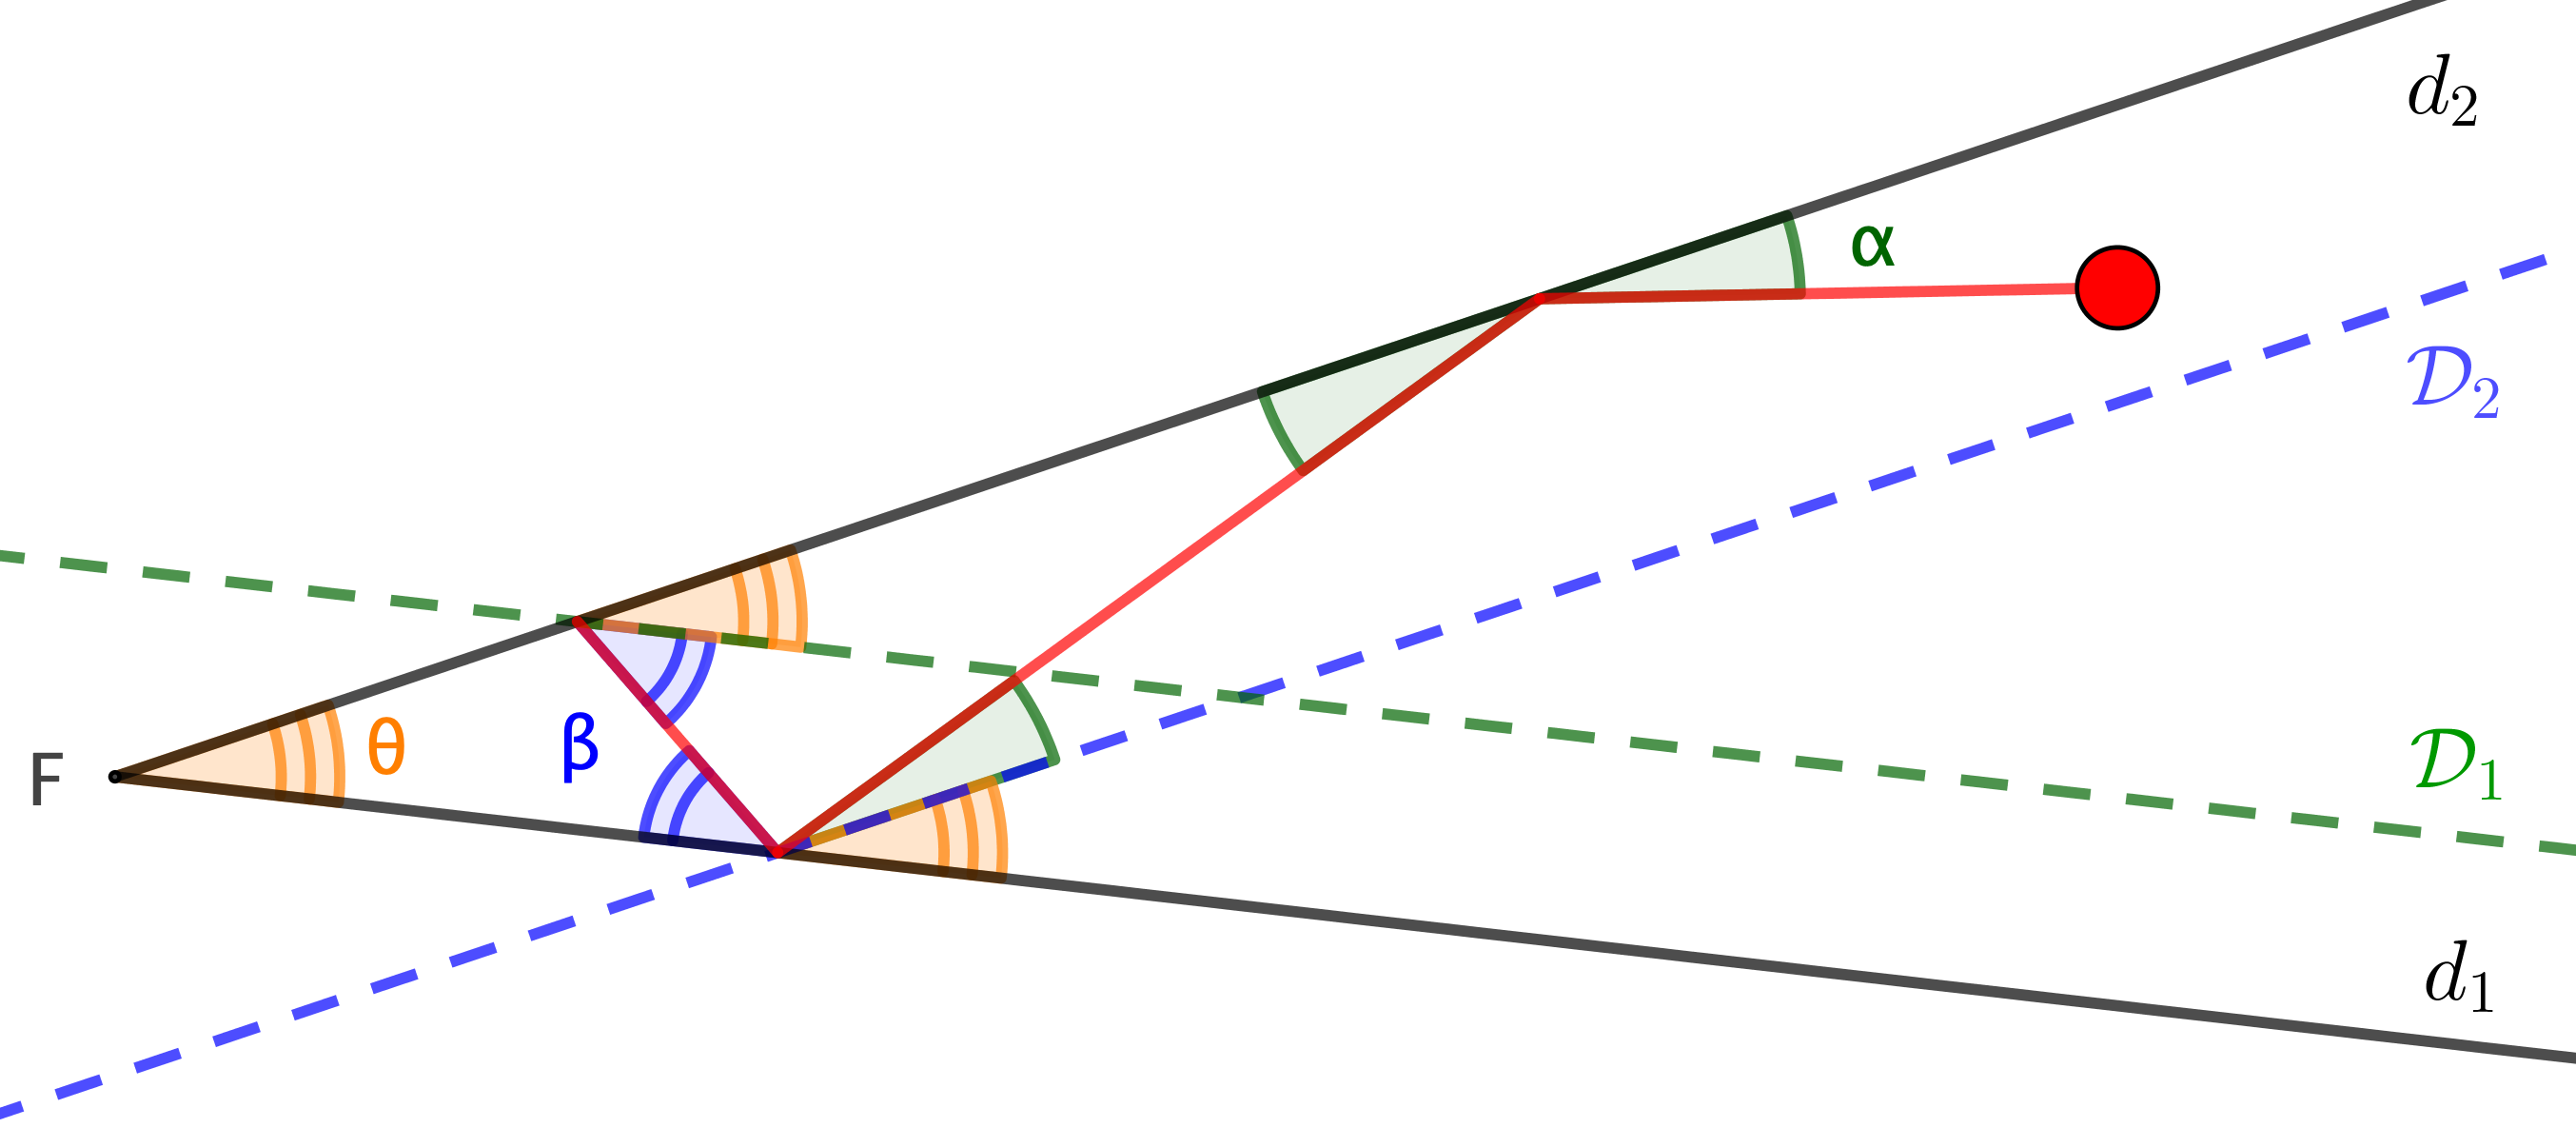
\includegraphics[width=12cm]{basic-math-pool/analysis-1.png}
	
	\itshape\small
	Situation n\textdegree1
	\label{situtation-1}
\end{center}


\medskip


Dans la 2\ieme{} situation ci-après, nous avons un rayon initial "allant à l'opposé de $F$" et faisant  avec la direction de $\geoset*{d}{2}$ un angle géométrique $\alpha \in \intervalO{0}{\frac{\pi}{2}}$ , puis au bout de deux rebonds, nous obtenons un rayon "allant à l'opposé de $F$" avec un angle géométrique mesurant $\alpha - 2\theta$ relativement à la direction de $\geoset*{d}{2}$.


\medskip


\begin{center}
	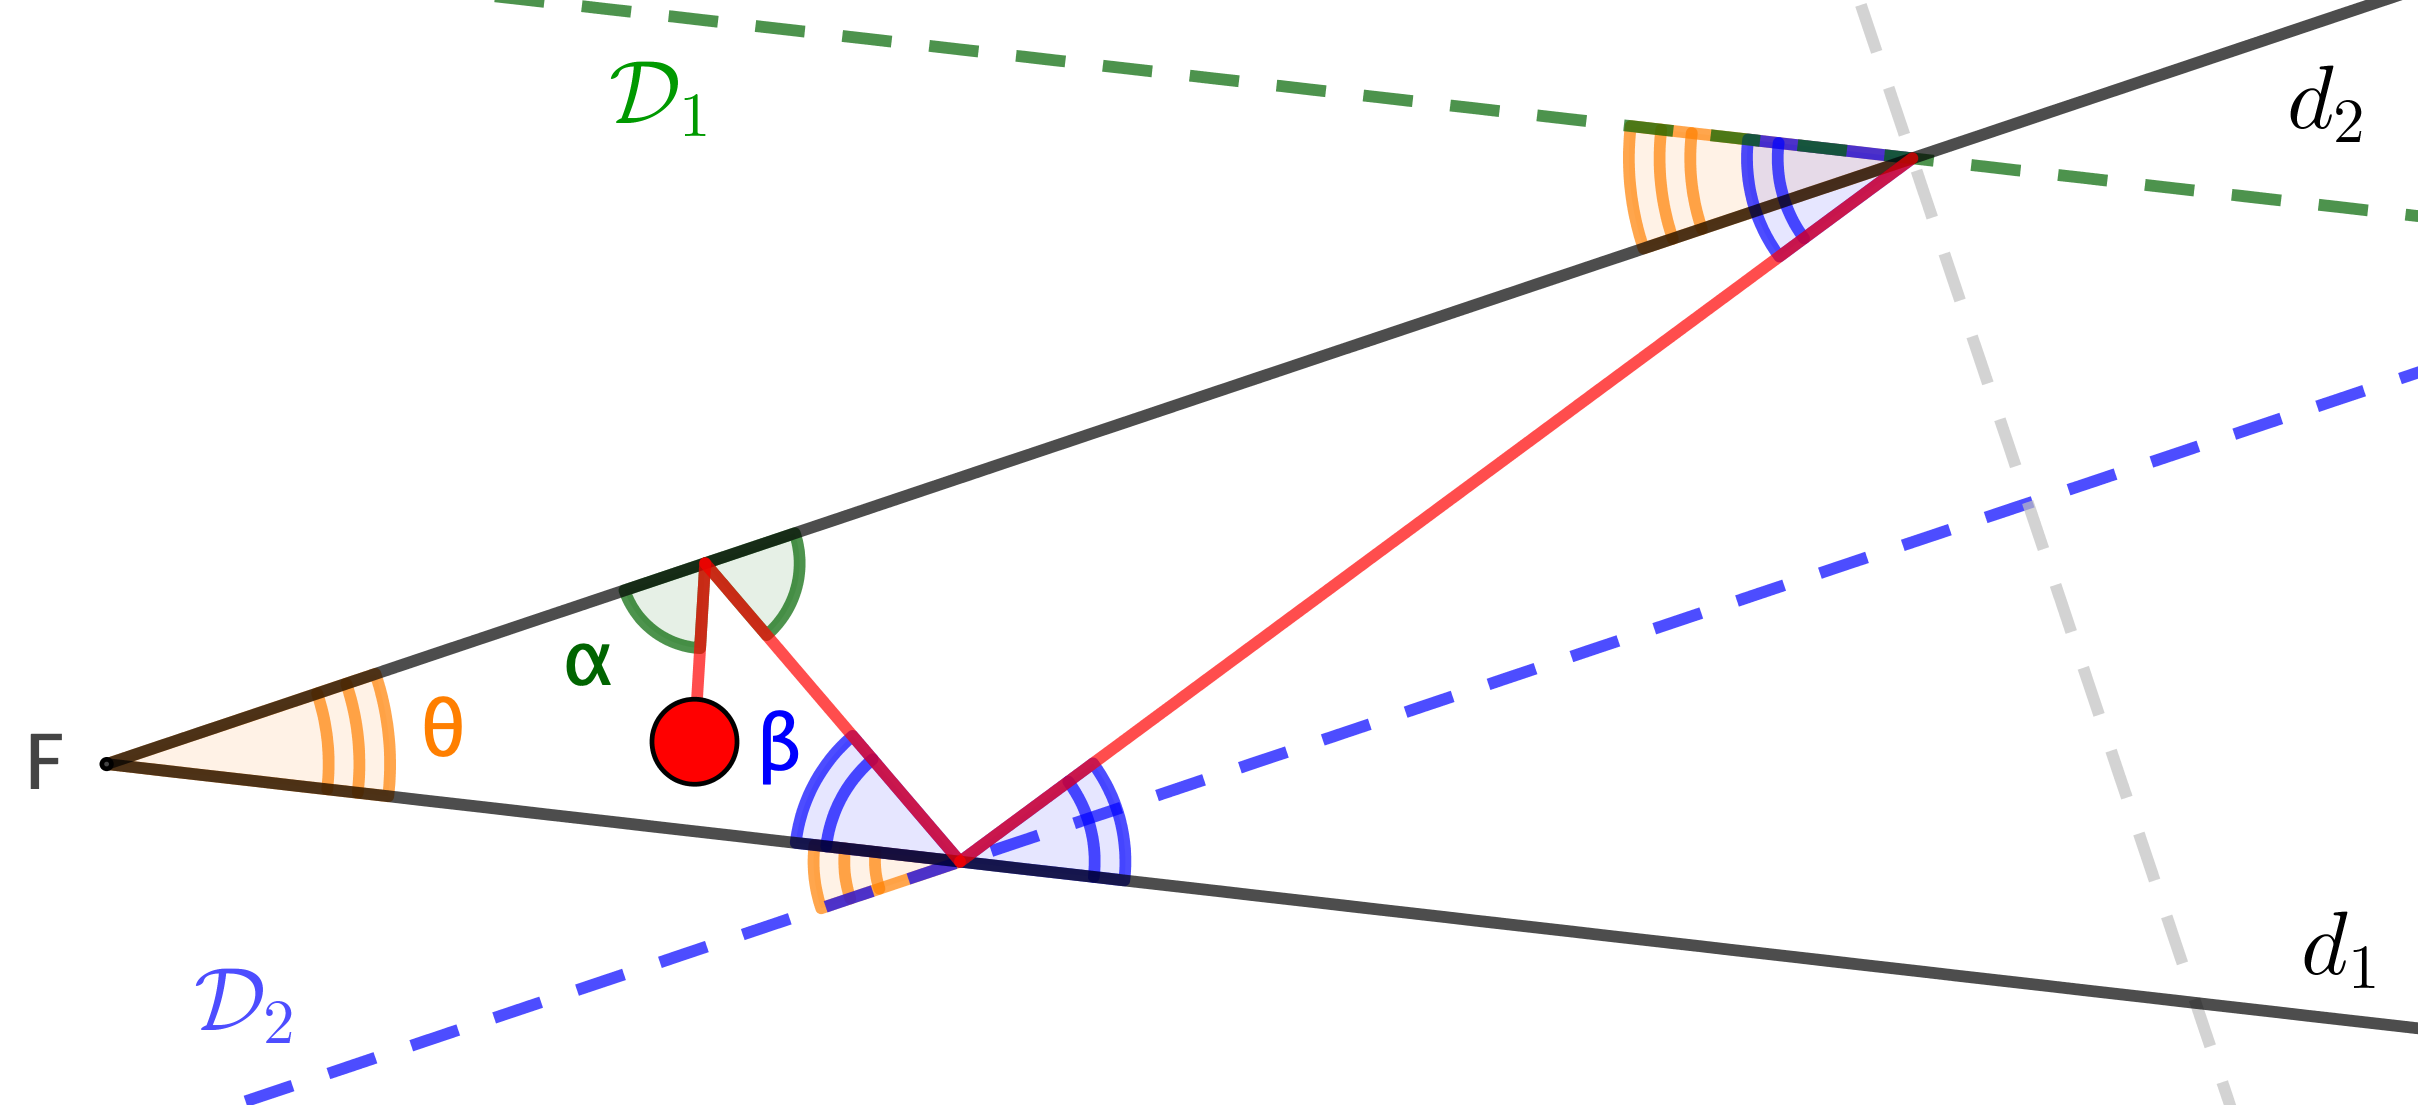
\includegraphics[width=12cm]{basic-math-pool/analysis-2.png}
	
	\itshape\small
	Situation n\textdegree2
	\label{situtation-2}
\end{center}


\medskip

Imaginons que notre bille soit d'abord confrontée à la situation n\textdegree1. Au bout de deux rebonds, l'angle relativement à $\geoset*{d}{2}$ passe de $\alpha_0 = \alpha$ à $\alpha_1 = \alpha + 2 \theta$. Une suite successive de situations n\textdegree1 va donc faire augmenter l'angle par rapport à la direction de $\geoset*{d}{2}$. Il arrivera donc un moment où la situation n\textdegree2 arrivera, excepté si l'on obtient un rebond perpendiculaire à $\geoset*{d}{2}$. Nous ignorons ici ce cas qui sera géré dans notre démonstration.

Une fois que la situation n\textdegree2 se présente, nous avons des angles de plus en plus petit relativement à $\geoset*{d}{2}$ jusqu'à arriver au dernier rebond possible après lequel la bille s'éloignera indéfiniment. Voilà une explication partielle du phénomène.